\section{Case Study 1} \label{moreno:sec:case1}

\begin{figure}

\centering
\subfigure[\footnotesize best-effort MPI architecture]{
  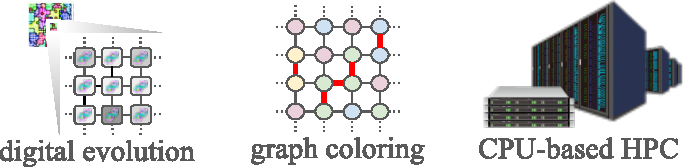
\includegraphics[width=\linewidth]{img/cpu-domain}
  \label{moreno:fig:cpu:architecture}
}

\vspace{2ex}
\centering
\subfigure[\footnotesize best-effort scaling performance]{
  
\includegraphics[width=\linewidth]{bindle/bindle-2026-05-16-perf-quality/bindle/teeplots/2026-05-16-perf-quality/col=panel+hue=executable+kind=line+row=asynchronicity-mode+viz=perf-quality-combined+x=ncpus+y=value+ext=.pdf}
  \label{moreno:fig:cpu:performance}
}

\vspace{2ex}

\subfigure[\footnotesize producer-consumer anomaly]{
  
\includegraphics[width=0.4\linewidth]{bindle/bindle-2026-05-15-mp-vs-mt-beleagurement/bindle/teeplots/2026-05-15-mp-vs-mt-beleagurement/col=multiprocessing+hue=hostname+kind=line+style=indexx+viz=relplot+x=type+y=count-per-second+ext=.pdf}%
  
\includegraphics[width=0.2\linewidth]{bindle/bindle-2026-05-15-mp-vs-mt-beleagurement/bindle/teeplots/2026-05-15-mp-vs-mt-beleagurement/hue=hostname+kind=box+viz=catplot+x=hostname+y=updates-per-second+ext=.pdf}%
  
\includegraphics[width=0.35\linewidth,angle=90]{bindle/bindle-2026-05-15-mp-vs-mt-beleagurement-ts/bindle/teeplots/2026-05-15-mp-vs-mt-beleagurement-ts/hue=special+kind=line+row=special+viz=relplot+x=rank3+y=updates-per-sec+ext=.pdf}
  \label{moreno:fig:cpu:producer-consumer}
}

\vspace{2ex}

\subfigure[\footnotesize producer-consumer anomaly]{
  
\includegraphics[width=0.5\linewidth]{bindle/bindle-2026-05-16-weak-scaling/bindle/teeplots/2026-05-16-weak-scaling/col=metric+cpus_per_node=1+hue=significance+kind=strip+marker=x+num_simels_per_cpu=1+row=kind+viz=catplot+x=num-processes+y=value+ext=.pdf}
  \label{moreno:fig:cpu:producer-consumer}
}

\vspace{2ex}

\subfigure[\footnotesize lac-417 node anomaly]{
  
\includegraphics[width=\linewidth]{bindle/bindle-2026-05-16-lac-417/bindle/teeplots/2026-05-16-lac-417/col=metric+hue=significance+kind=strip+marker=x+row=kind+viz=catplot+x=0-sans-lac-417-1-with-lac-417+y=value+ext=.pdf}
  \label{moreno:fig:cpu:lac417}
}

\vspace{2ex}

\caption{
\textbf{TODO.}
\footnotesize
TODO
}
\label{moreno:fig:cpu}
\end{figure}


The Message Passing Interface (MPI) standard \cite{gropp1996high} represents the mainstay for high-performance computing applications.
This standard exposes communication primitives directly to the end user.
MPI's nonblocking communication primitives, in particular, are sufficient to program distributed computations with relaxed synchronization requirements.
Although it's explicit, the imperative nature of the MPI protocols enables precise control over execution; unfortunately it also poses significant expense in terms of programmability.
This cost manifests in terms of reduced programmer productivity and software quality, while increasing domain knowledge requirements and the effort required to tune for performance due to program brittleness \cite{gu2019comparative, tang2014mpi}.

In response to programmability concerns, many frameworks have arisen to offer useful parallel and distributed programming abstractions.
Task-based frameworks such as Charm++ \cite{kale1993charm++}, Legion \cite{bauer2012legion}, Cilk \cite{blumofe1996cilk}, and Threading Building Blocks (TBB) \cite{reinders2007intel} describe the dependency relationships among computational tasks and associated data and rely on an associated runtime to automatically schedule and manage execution.
These frameworks assume a deterministic relationship between tasks.
In a similar vein, programming languages and extensions like Unified Parallel C (UPC) \cite{el2006upc} and Chapel \cite{chamberlain2007parallel} rely on programmers to direct execution, but equip them with powerful abstractions, such as global shared memory.
However, Chapel's memory model explicitly forbids data races and UPC ultimately relies on a barrier model for data transfer.

To bridge these shortcomings, we employ a new software framework, the Conduit C++ Library for Best-Effort High Performance Computing \cite{moreno2021conduit}.
The Conduit library provides tools to perform best-effort communication in a flexible, intuitive interface and uniform inter-operation of serial, parallel, and distributed modalities.
Although Conduit currently implements distributed functionality via MPI intrinsics, in future work we will explore lower-level protocols like InfiniBand Unreliable Datagrams \cite{kashyap2006ip, koop2007high}.
